\chapter{Кривизны}
\label{chap:surface-curvature}

Из предыдущей главы мы знаем, что касательная плоскость к поверхности имеет с ней касание первого порядка.
В частности, вплоть до первого порядка все поверхности выглядят одинаково вблизи одной точки.
Для приближений второго порядка, появляются различия, о которых и пойдёт речь.


\section{Касательно-нормальные координаты}
\label{sec:lmn}
\index{касательно-нормальные координаты}

{\sloppy

Выберем точку $p$ на гладкой ориентированной поверхности~$\Sigma$;
пусть $\Norm$ --- её поле нормалей.
Рассмотрим систему координат $(x,y,z)$ с началом в точке $p$, чтобы касательная плоскость $\T_p$ стала горизонтальной, а ось $z$ была направлена по $\Norm(p)$.
Такие координаты будут называться {}\emph{касательно-нормальными}. 
Согласно \ref{ex:vertical-tangent},
окрестность $p$ в $\Sigma$ можно задать графиком $z=f(x,y)$ гладкой функции,
при этом
\begin{align*}
f(0,0)&=0,
&
f_x(0,0)&=0,
&
f_y(0,0)&=0.
\end{align*}
Первое равенство означает, что $p=(0,0,0)$ лежит на графике, а два других --- то, что касательная плоскость в $p$ горизонтальна.

}

\begin{wrapfigure}[7]{o}{42 mm}
\vskip-3mm
\centering
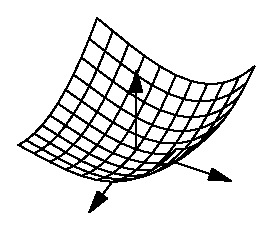
\includegraphics{asy/paraboloid}
\vskip-3mm
\end{wrapfigure}

Пусть
\begin{align*}
\ell&=f_{xx}(0,0),
\\
m&=f_{xy}(0,0)=f_{yx}(0,0),
\\
n&=f_{yy}(0,0).
\end{align*}
\textit{Ряд Тейлора} $f$ в $(0,0)$ до второго порядка записывается как
\[f(x,y)=\tfrac12(\ell\cdot x^2+2\cdot m\cdot x\cdot y+n\cdot y^2)+o(x^2+y^2).\phantom{f(x,y)=\tfrac12(\ell\cdot x^2+}\]
Значения $\ell$, $m$ и $n$ полностью определяются этим уравнением.\index{10lmn@$\ell$, $m$, $n$ (компоненты матрицы Гессе)}
График многочлена Тейлора 
\[z=\tfrac12\cdot(\ell\cdot x^2+2\cdot m\cdot x\cdot y+n\cdot y^2)\]
называется \index{соприкасающийся параболоид}\emph{соприкасающимся параболоидом}.
Он имеет \index{порядок касания}\emph{второй порядок касания} с $\Sigma$ в~$p$.

Далее заметим, что 
\[\ell\cdot x^2+2\cdot m\cdot x\cdot y+n\cdot y^2=\langle M_p\cdot (\begin{smallmatrix}
x\\y
\end{smallmatrix}), (\begin{smallmatrix}
x\\y
\end{smallmatrix})\rangle,\]
где 
\[M_p=\begin{pmatrix}
 \ell
 &m
 \\
 m
 &n
 \end{pmatrix}
=\begin{pmatrix}
 f_{xx}(0,0)
 &f_{xy}(0,0)
 \\
 f_{yx}(0,0)
 &f_{yy}(0,0)
 \end{pmatrix}.
\eqlbl{eq:hessian}
\]
--- так называемая \index{матрица Гессе}\emph{матрица Гессе} $f$ в точке $(0,0)$,\index{10m@$M_p$ (матрица Гессе)}


\section{Главные кривизны}\label{sec:Principal curvatures}

Касательно-нормальные координаты почти однозначно определяются точкой на поверхности;
они единственны с точностью до вращения плоскости $(x,y)$.
При вращении этой плоскости  матрица Гессе $M_p$ переписывается в новом базисе.

Поскольку матрица $M_p=\left(\begin{smallmatrix}
 \ell
 &m
 \\
 m
 &n
 \end{smallmatrix}\right)$ 
симметрична, по спектральной теореме (\ref{thm:spectral}), её можно диагонализовать ортогональной матрицей.
То есть, вращая плоскость $(x,y)$, можно добиться того, что $m=0$.
В этом случае,
\[M_p=\begin{pmatrix}
 k_1
 &0
 \\
 0
 &k_2
 \end{pmatrix},
\]
числа $k_1$ и $k_2$  на диагонали называются \index{главные кривизны и направления}\emph{главными кривизнами} $\Sigma$ в точке $p$;\index{10k@$k_1$, $k_2$ (главные кривизны)}
их можно обозначать $k_1(p)$ и $k_2(p)$, или $k_1(p)_\Sigma$ и $k_2(p)_\Sigma$, если нужно подчеркнуть, что они вычисляются в точке $p$ для поверхности~$\Sigma$.
Если не указано обратное, мы будем считать, что 
\[k_1\le k_2.\]

{\sloppy

Если в этих координатах $\Sigma$ локально задаётся графиком $z\z=f(x,y)$, то 
\[f(x,y)=\tfrac12\cdot(k_1\cdot x^2+k_2\cdot y^2)+o(x^2+y^2).\]

}

Главные кривизны можно также определить как собственные значения матрицы $M_p$.
Собственные направления $M_p$ называются {}\emph{главными направлениями} $\Sigma$ в точке~$p$.
Если $k_1(p)\ne k_2(p)$, то в точке $p$ есть ровно два главных направления, которые перпендикулярны друг другу;
если же $k_1(p) = k_2(p)$, то все касательные направления в точке $p$ главные.

Если обратить ориентацию $\Sigma$, то главные кривизны поменяют свои знаки и индексы:
$k_1$ превратиться в $-k_2$, а $k_2$ в $-k_1$.

Гладкая кривая на поверхности $\Sigma$, всё время идущая в главных направлениях, называется \index{линия кривизны}\emph{линией кривизны}~$\Sigma$.
Если $k_1(p)\z\ne k_2(p)$, то в точке $p$ существует карта $(u,v)\mapsto s(u,v)$ с координатными линиями, образованными линиями кривизны (это вытекает из \ref{ex:lin-ind-chart}), при этом $s_u\perp s_v$, ведь главные направления перпендикулярны.

\begin{thm}{Упражнение}\label{ex:line-of-curvature}
Пусть $\Sigma$ --- гладкая поверхность, зеркально-симметричная относительно плоскости $\Pi$.
Допустим, что $\Sigma$ и $\Pi$ пересекаются по гладкой кривой~$\gamma$.
Покажите, что $\gamma$ --- линия кривизны.
\end{thm}


\section{Ещё кривизны}\label{sec:More curvatures}

Пусть $p$ --- точка на ориентированной гладкой поверхности~$\Sigma$.
Напомним, что $k_1(p)$ и $k_2(p)$ обозначают главные кривизны в точке~$p$.

Произведение 
\[K(p)=k_1(p)\cdot k_2(p)\]
называется \index{10k@$K$ (гауссова кривизна)}\index{гауссова кривизна}\emph{гауссовой кривизной} в точке~$p$.
Её можно обозначать $K$, $K(p)$ и даже $K(p)_\Sigma$, если хочется указать и точку и поверхность.

Поскольку определитель равен произведению собственных значений, получаем, что
\[K=\ell\cdot n-m^2,\]
где 
$M_p=
(\begin{smallmatrix}
\ell&m
\\
m&n
\end{smallmatrix}
)$
--- матрица Гессе.

Отметим, что обращение ориентации $\Sigma$ не меняет гауссову кривизну,
и, значит, она определена и для неориентированных поверхностей.

\begin{thm}{Упражнение}\label{ex:gauss+orientable}
Покажите, что любая поверхность с положительной гауссовой кривизной ориентируема. 
\end{thm}

Сумма \index{10h@$H$ (средняя кривизна)}
\[H(p)=k_1(p)+ k_2(p)\] 
называется \index{кривизна}\index{средняя кривизна}\emph{средней кривизной}%
\footnote{Некоторые авторы определяют её как $\tfrac12\cdot(k_1(p)+ k_2(p))$ --- среднее значение главных кривизн.
Это лучше подходит к названию, но оказывается не удобно.}
в точке~$p$.
Если нужно, её можно обозначать как $H(p)_\Sigma$.
Можно думать, что средняя кривизна --- это след матрицы Гессе $M_p=
(\begin{smallmatrix}
\ell&m
\\
m&n
\end{smallmatrix}
)$;
то есть
\[H=\ell+n.\] 
Обращение ориентации $\Sigma$ меняет знак её средней кривизны.

Поверхность с нулевой средней кривизной называется \index{минимальная поверхность}\emph{минимальной}.

\begin{thm}{Упражнение}\label{ex:re-scale-surface-curvature}
Пусть $\Sigma$ --- ориентированная поверхность, а $\Sigma_{\lambda}$ --- её гомотетия с коэффициентом $\lambda > 0$; то есть $\Sigma_{\lambda}$ состоит из точек $\lambda \cdot x$, где $x \in \Sigma$.
Покажите, что
\[K(\lambda\cdot p)_{\Sigma_{\lambda}}
= \tfrac{1}{\lambda^2}\cdot K(p)_{\Sigma}
\quad\text{и}\quad
H(\lambda \cdot p)_{\Sigma_{\lambda}} = \tfrac1\lambda\cdot H(p)_{\Sigma}\]
для любой точки $p\in \Sigma$.  
\end{thm}


\section{Оператор формы}\label{sec:shape}

В следующих определениях используется понятие производной по направлению и дифференциала, см.~\ref{sec:dirder} и~\ref{sec:differential}.

Пусть $p$ --- точка на гладкой поверхности $\Sigma$ с ориентацией, заданной полем нормалей $\Norm$,
и пусть $\vec w$ --- касательный вектор при $p$.
\index{оператор формы}\emph{Оператор формы}%
\footnote{
Следующие билинейные формы на касательной плоскости  
\begin{align*}
\mathrm{I}(\vec v,\vec w)&=\langle\vec v,\vec w\rangle,
&
\mathrm{II}(\vec v,\vec w)&=\langle\Shape\vec v,\vec w\rangle,
&
\mathrm{III}(\vec v,\vec w)&=\langle\Shape\vec v,\Shape\vec w\rangle
\end{align*}
называются \index{фундаментальная форма}\emph{первой, второй и третьей фундаментальными формами}, соответственно.
Исторически, эти формы были введены до оператора формы, но мы вовсе не станем их рассматривать.
} от $\vec w$ определяется как
\[\Shape_p\vec w=-D_{\vec w}\Norm.\]
Его также можно определить как
\[\Shape=-d\Norm,\eqlbl{eq:shape=-L}\] 
где $d\Norm$ --- дифференциал сферического отображения $\Norm\:\Sigma\to\mathbb{S}^2$; то есть $d_p\Norm(\vec v)=(D_{\vec v}\Norm)(p)$.

Напомним, что $d_p\Norm$ --- это линейное отображение $\T_p\Sigma\to \T_{\Norm(p)}\mathbb{S}^2$.
Заметим, что $\T_p\Sigma$ совпадает с $\T_{\Norm(p)}\mathbb{S}^2$, ведь обе плоскости перпендикулярны $\Norm(p)$.
Поэтому $\Shape_p$ действительно является линейным оператором $\T_p\to \T_p$ (это также будет следовать из \ref{thm:shape-chart}).

Для точки $p\in \Sigma$, оператор формы от касательного вектора $\vec w\in \T_p$ будет обозначаться как $\Shape\vec w$, если из контекста ясно, о какой базовой точке $p$ и о какой поверхности идет речь;
в противном случае можно писать 
\[\Shape_p(\vec w)\quad\text{или}\quad \Shape_p(\vec w)_\Sigma.\]


\begin{thm}{Теорема}\label{thm:shape-chart}
Пусть $(u,v)\mapsto s(u,v)$ --- гладкое отображение на гладкую поверхность $\Sigma$ с полем нормалей $\Norm$.
Тогда 
\begin{align*}
\langle \Shape(s_u), s_u\rangle 
&=\langle s_{uu},\Norm\rangle,
&
\langle \Shape(s_v), s_u\rangle 
&=\langle s_{uv},\Norm\rangle,
\\
\langle \Shape(s_u), s_v\rangle 
&=\langle s_{uv},\Norm\rangle,
&
\langle \Shape(s_v), s_v\rangle 
&=\langle s_{vv},\Norm\rangle,
\\
\langle \Shape(s_u), \Norm\rangle 
&=0,
&
\langle \Shape(s_v), \Norm\rangle 
&=0
\end{align*}
для любых $(u,v)$.

\end{thm}

\parbf{Доказательство.}
Будем использовать сокращение $\Norm=\Norm(u,v)$ для $\Norm(s(u,v))$,
так что 
\[
\begin{aligned}
\Shape(s_u)&=-D_{s_u}\Norm=-\Norm_u,
&
\Shape(s_v)&=-D_{s_v}\Norm=-\Norm_v.
\end{aligned}
\eqlbl{eq:shape=norm_u}
\]

Поскольку $\Norm$ --- единичный вектор, ортогональный к $s_u$ и $s_v$,
\begin{align*}
\langle \Norm,s_u\rangle&\equiv0,
&
\langle \Norm,s_v\rangle&\equiv0,
&
\langle \Norm,\Norm\rangle&\equiv1.
\end{align*}
Взяв частные производные этих тождеств, получим
\begin{align*}
\langle \Norm_u,s_u\rangle+\langle \Norm,s_{uu}\rangle&=0,
&
\langle \Norm_v,s_u\rangle+\langle \Norm,s_{uv}\rangle&=0,
\\
\langle \Norm_u,s_v\rangle+\langle \Norm,s_{uv}\rangle&=0,
&
\langle \Norm_v,s_v\rangle+\langle \Norm,s_{vv}\rangle&=0,
\\
2\cdot\langle \Norm_u,\Norm\rangle&=0,
&
2\cdot\langle \Norm_v,\Norm\rangle&=0.
\end{align*}
Остаётся подставить сюда выражения из \ref{eq:shape=norm_u}.
\qeds


\begin{thm}{Упражнение}\label{ex:self-adjoint}
Покажите, что оператор формы \index{самосопряжённый оператор}\emph{самосопряжён}; то есть
\[\langle \Shape\vec u,\vec v\rangle=\langle \vec u,\Shape\vec v\rangle\]
для любых $\vec u,\vec v\in\T_p$.
\end{thm}

Обозначим стандартный базис в $\mathbb{R}^3$ как $\vec i$, $\vec j$ и $\vec k$.\index{10i@$\vec i$, $\vec j$, $\vec k$ (стандартный базис)}
Напомним, что компоненты $\ell$, $m$ и $n$ матрицы Гессе определены в~\ref{sec:lmn}.

\begin{thm}{Следствие}\label{cor:Shape(ij)}
Пусть $z=f(x,y)$ --- локальное представление гладкой поверхности $\Sigma$ в касательно-нормальных координатах при точке~$p$,
и пусть $(\begin{smallmatrix}
\ell&m\\ m&n
\end{smallmatrix})$ --- её матрица Гессе.
Тогда 
\begin{align*}
\Shape\vec i&=\ell\cdot \vec i+m\cdot \vec j,
&
\Shape\vec j&=m\cdot \vec i+n\cdot\vec j,
\end{align*}
для стандартного базиса $\vec i,\vec j,\vec k$.
Иначе говоря, оператор формы задаётся умножением на матрицу Гессе.
\end{thm}

Это следствие обнажает связь между кривизнами и оператором формы.
Главные кривизны $\Sigma$ в точке $p$ --- это собственные значения $\Shape_p$, главные направления --- это собственные направления $\Shape_p$, гауссова кривизна --- это определитель $\Shape_p$, а средняя кривизна --- это след $\Shape_p$.

Поскольку матрица Гессе симметрична, из следствия получаем, что оператор формы самосопряжён;
это решает упражнение \ref{ex:self-adjoint}.

\parbf{Доказательство.}
Заметим, что $s\:(u,v)\mapsto (u,v,f(u,v))$ --- карта на $\Sigma$ при~$p$.
Кроме того, 
\begin{align*}
s_u(0,0)&=\vec i,
&
s_v(0,0)&=\vec j,
&
\Norm(0,0)&=\vec k,
\\
s_{uu}(0,0)&=\ell\cdot \vec k,
&
s_{uv}(0,0)&=m\cdot \vec k,
&
s_{vv}(0,0)&=n\cdot \vec k.
\end{align*}
Остаётся применить \ref{thm:shape-chart}.
\qeds


\begin{thm}{Следствие}\label{cor:intK}
Пусть $\Sigma$ --- гладкая поверхность с полем нормалей $\Norm$.
Допустим, что сферическое отображение $\Norm\:\Sigma\to\mathbb{S}^2$ инъективно.
Тогда 
\[\iint_\Sigma|K|=\area[\Norm(\Sigma)].\]
\end{thm}

{\sloppy

\parbf{Доказательство.}
Выберем ортонормированный базис в $\T_p$, в главных направлениях.
Тогда оператор формы выражается матрицей 
$(\begin{smallmatrix}
 k_1
 &0
 \\
 0
 &k_2
\end{smallmatrix})$.

}

Поскольку $\Shape_p=-d_p\Norm$, из \ref{cor:Shape(ij)} получаем, что
\[\jac_p\Norm=|\det(\begin{smallmatrix}
 k_1
 &0
 \\
 0
 &k_2
 \end{smallmatrix})|=|K(p)|.\]
Остаётся применить формулу площади (\ref{prop:surface-integral}).
\qeds



\begin{thm}{Упражнение}\label{ex:normal-curvature=const}
Пусть $\Sigma$ --- гладкая поверхность с полем нормалей $\Norm$, и её главные кривизны  равны 1 во всех точках.

\begin{subthm}{ex:normal-curvature=const:a}
Докажите, что $\Shape_p(\vec w)=\vec w$ для любых $p\in\Sigma$ и $\vec w\in \T_p\Sigma$.
\end{subthm}

\begin{subthm}{ex:normal-curvature=const:b}
Докажите, что точка $q\z= p+\Norm(p)$ постоянна; то есть точка $q$ не зависит от выбора $p\in\Sigma$.
Выведите отсюда, что $\Sigma$ является подмножеством единичной сферы с центром в~$q$.
\end{subthm}

\end{thm}

{\sloppy

\begin{thm}{Продвинутое упражнение}\label{ex:normal-curvature=0}
Пусть $\Sigma$ --- гладкая поверхность, $\Norm$ --- её поле нормалей, и $Z_0\subset \Sigma$ --- связное множество с нулевым оператором формы. 
Докажите, что $Z_0$ лежит в плоскости.
\end{thm}

}

{}\emph{Угол} между двумя ориентированными поверхностями в точке их пересечения $p$ определяется как угол между их нормалями в~$p$.

\begin{thm}{Упражнение}\label{ex:shape-curvature-line}
Предположим, что две гладкие ориентированные поверхности $\Sigma_1$ и $\Sigma_2$ пересекаются по гладкой кривой~$\gamma$ под постоянным углом.
Пусть $\gamma$ --- линия кривизны на $\Sigma_1$.
Докажите, что $\gamma$ также является линией кривизны на $\Sigma_2$.

Выведите отсюда, что если гладкая поверхность $\Sigma$ пересекает плоскость или сферу вдоль гладкой кривой $\gamma$ под постоянным углом, то $\gamma$ является линией кривизны на~$\Sigma$.
\end{thm}

\begin{thm}{Упражнение}\label{ex:equidistant}
Пусть $\Sigma$ --- замкнутая гладкая поверхность с ориентацией, определённой полем нормалей $\Norm$.

\begin{subthm}{ex:equidistant:smooth}
Докажите, что множество 
\[\Sigma_t=\set{p+t\cdot \Norm(p)}{p\in\Sigma}\] 
является гладкой поверхностью при всех $t$ достаточно близко к нулю.
\end{subthm}

\begin{subthm}{ex:equidistant:area}
Докажите, что для всех $t$, достаточно близких к нулю, справедливо равенство
\[\area\Sigma_t=\area\Sigma-t\cdot \iint_\Sigma H+t^2\cdot \iint_\Sigma K,\]
где $H$ и $K$ обозначают среднюю и гауссову кривизну~$\Sigma$.
\end{subthm}

\end{thm}



\begin{thm}{Продвинутое упражнение}\label{ex:flat-plane}{\sloppy
Пусть $\Sigma$ --- гладкая ориентированная поверхность, параметризованная координатным прямоугольником $(u,v)\mapsto s(u,v)$,
и пусть $\vec u=\tfrac{s_u}{|s_u|}$, $\vec v=\tfrac{s_v}{|s_v|}$ и $\Norm(u,v)$ --- нормаль в точке $s(u,v)$.

}

Предположим, что $\vec u$ и $\vec v$ --- поля главных направлений;
пусть $0$ и $k\z=k(u,v)$ будут их главными кривизнами,
при этом $k$ не обращается в ноль и $|s_u|=1$ на одной из $u$-координатных линий.

\begin{subthm}{ex:flat-plane:orthonormal}
Докажите, что $\Norm(u,v)$, $\vec u(u,v)$ и $\vec v(u,v)$ образуют ортонормированный базис для любых $(u,v)$.
\end{subthm}

\begin{subthm}{ex:flat-plane:depend}
Докажите, что $\Norm(u,v)$, $\vec u(u,v)$ и $\vec v(u,v)$ зависят только от $v$.
Выведите отсюда, что $u$-координатные линии являются отрезками.
\end{subthm}

\begin{subthm}{ex:flat-plane:depend-u}
Докажите, что $s_{uu}$ пропорционален $s_u$ во всех точках.
Выведите отсюда, что $|s_u|=1$ во всех точках.
\end{subthm}

\begin{subthm}{ex:flat-plane:linear}
Докажите, что при фиксированном $v_0$ значение $\tfrac1{k(u,v_0)}$ линейно зависит от $u$.
\end{subthm}

\end{thm}

Упражнение содержит основную часть доказательства следующей теоремы:
\textit{Любая открытая поверхность с нулевой гауссовой кривизной является \index{цилиндрическая поверхность}\emph{цилиндрической}}\,;
то есть она заметается семейством параллельных прямых.
Упражнения \ref{ex:lin-ind-chart} и \ref{ex:line-cylinder} иллюстрирует другие части этого доказательства.
Упомянутая теорема была изначально доказана Алексеем Погореловым \cite[II §3 теорема 2]{pogorelov1956} в гораздо более общих предположениях и была неоднократно переоткрыта \cite{hartman-nirenberg,massey1962}.


\chapter{Кривые на поверхности}\label{chap:Curves in a surface}

\section{Базис Дарбу}\label{sec:Darboux}

\begin{wrapfigure}{r}{42 mm}
\vskip-20mm
\centering
\begin{lpic}[t(-0mm),b(0mm),r(0mm),l(0mm)]{asy/paraboloid+curve(1)}
\lbl[ul]{34,14;$\tan$}
\lbl[b]{20,43;$\Norm$}
\lbl[bl]{38,35;$\mu$}
\end{lpic}
\vskip-0mm
\end{wrapfigure}

Пусть $\gamma$ --- гладкая кривая на гладкой ориентированной поверхности~$\Sigma$,
с полем нормалей $\Norm$.
Будем считать, что $\gamma$ параметризована длиной, а значит, $\tan(s)\z=\gamma'(s)$ --- её касательная индикатриса.
Далее будем пользоваться сокращением $\Norm(s)\z=\Norm(\gamma(s))$.

Единичные векторы $\tan(s)$ и $\Norm(s)$ ортогональны.
Поэтому существует единственный единичный вектор $\mu(s)$\index{10tmn@$\tan$, $\mu$, $\Norm$ (базис Дарбу)}, такой что 
$\tan(s),\mu(s),\Norm(s)$ образуют ориентированный ортонормированный базис, он называется \index{базис Дарбу}\emph{базис Дарбу} кривой $\gamma$ на~$\Sigma$.

Поскольку $\T_{\gamma(s)}\z\perp\Norm(s)$, вектор $\mu(s)$ касается $\Sigma$ в точке $\gamma(s)$.
На самом деле, $\mu(s)$ можно получить повернув $\tan(s)$ в $\T_{\gamma(s)}$ против часовой стрелки на угол $\tfrac\pi2$.
Этот вектор также можно определить через векторное произведение $\mu(s)\z\df\Norm(s)\times \tan(s)$.


Поскольку у $\gamma$ единичная скорость, $\gamma''\perp \gamma'$ (см. \ref{prop:a'-pertp-a''}).
В частности, $\gamma''$ можно записать как линейную комбинацию $\mu$ и $\Norm$;
то есть \index{10k@$k_g$ геодезическая кривизна}\index{10k@$k_n$ (нормальная кривизна)}
\[\gamma''(s)=k_g(s)\cdot \mu(s)+k_n(s)\cdot\Norm(s).\]
Величины $k_g(s)$ и $k_n(s)$ называются соответственно \index{кривизна}\index{геодезическая!кривизна}\emph{геодезической} и \index{нормальная!кривизна}\emph{нормальной кривизной} кривой $\gamma$ при $s$.
Поскольку базис $\tan(s)$, $mu(s)$, $\Norm(s)$ ортонормирован, эти кривизны переписываются через скалярные произведения
\begin{align*}
k_g(s)&=\langle \gamma''(s),\mu(s)\rangle= 
&
k_n(s)&=\langle \gamma''(s),\Norm(s)\rangle=
\\
&=\langle \tan'(s),\mu(s)\rangle,
&
&=\langle \tan'(s),\Norm(s)\rangle.
\end{align*}

Продифференцировав $0=\langle \tan(s),\Norm(s)\rangle$, получим
\begin{align*}
0&=\langle \tan(s),\Norm(s)\rangle'=
\\
&=\langle \tan'(s),\Norm(s)\rangle+\langle \tan(s),\Norm'(s)\rangle=
\\
&=k_n(s)+\langle \tan(s),D_{\tan(s)}\Norm\rangle.
\end{align*}
И, применив определение оператора формы,
получим следующее.

\begin{thm}{Предложение}\label{prop:normal-shape}
Пусть $\gamma$ --- гладкая кривая с единичной скоростью на гладкой поверхности~$\Sigma$, $p=\gamma(s_0)$ и $\vec v=\gamma'(s_0)$.
Тогда 
\[k_n(s_0)=\langle \Shape_p(\vec v),\vec v\rangle,\]
где $k_n$ --- нормальная кривизна $\gamma$ при $s_0$, а $\Shape_p$ --- оператор формы в~точке~$p$.
\end{thm}

Согласно предложению, нормальная кривизна гладкой кривой на $\Sigma$ полностью определяется её вектором скорости~$\vec v$.
Поэтому нормальную кривизну в направлении $\vec v$ допустимо обозначать как $k_{\vec v}$\index{10k@$k_{\vec v}$ (нормальная кривизна)} и
\[k_{\vec v}=\langle \Shape_p(\vec v),\vec v\rangle\]
для любого единичного вектора $\vec v$ в $\T_p$.


\section{Формула Эйлера}

Пусть $p$ --- точка на гладкой поверхности~$\Sigma$.
Выберем касательно-нормальные координаты при $p$ с диагональной матрицей Гессе
\[M_p=\begin{pmatrix}
 k_1(p)
 &0
 \\
 0
 &k_2(p)
 \end{pmatrix}.
\]
Рассмотрим вектор ${\vec w}=a\cdot\vec i+b\cdot\vec j$ касательный в $p$.
Согласно \ref{cor:Shape(ij)},
\[
\langle \Shape\vec w,\vec w\rangle
=a^2\cdot k_1(p) +b^2\cdot k_2(p). 
\]
Поскольку $|{\vec w}|^2=a^2+b^2$, получаем следующее.

\begin{thm}{Наблюдение}\label{obs:k1-k2}
Для любой точки $p$ на ориентированной гладкой поверхности $\Sigma$,
главные кривизны $k_1(p)$ и $k_2(p)$ являются соответственно минимумом и максимумом нормальных кривизн в~точке $p$.
Более того, если $\theta$ --- угол между единичным вектором ${\vec w}\in\T_p$ и первым главным направлением, то 
\[k_{\vec w}(p)=k_1(p)\cdot(\cos\theta)^2+k_2(p)\cdot(\sin\theta)^2.\]

\end{thm}

Последнее тождество называется \index{формула Эйлера}\emph{формулой Эйлера}.

\begin{thm}{Упражнение}\label{ex:mean-curvature}
Покажите, что средняя кривизна $H(p)$ в точке~$p$ на гладкой поверхности равна сумме нормальных кривизн для любой пары ортогональных касательных направлений в $p$. 
\end{thm}

\begin{thm}{Упражнение}\label{ex:average}
Покажите, что $\tfrac38\cdot H(p)^2-\tfrac12\cdot K(p)$ равно среднему значению квадрата нормальных кривизн при $p$;
то есть среднему значению $k_{\vec w}^2$ для всех единичных векторов ${\vec w}\in\T_p$.
\end{thm}

{\sloppy

\begin{thm}{Теорема Мёнь\'{е}}
\label{thm:meusnier}
\index{теорема Мёнье}
Пусть $\gamma$ --- гладкая кривая на гладкой ориентированной поверхности~$\Sigma$, $p=\gamma(t_0)$, ${\vec v}\z=\gamma'(t_0)$ и $\alpha\z=\measuredangle(\Norm(p),\norm(t_0))$;
то есть $\alpha$ --- угол между нормалью к $\Sigma$ в точке $p$ и нормальным вектором в базисе Френе кривой $\gamma$ при~$t_0$.
Тогда 
\[\kur(t_0)\cdot\cos\alpha=k_{n}(t_0);\]
здесь $\kur(t_0)$ и $k_n(t_0)$ --- кривизна и нормальная кривизна $\gamma$ при $t_0$, соответственно. 
\end{thm}

}

\parbf{Доказательство.}
Так как $\gamma''=\tan'=\kur\cdot \norm$, 
\begin{align*}
k_{n}(t_0)&=\langle\gamma''(t_0),\Norm(p)\rangle=
\\
&=\kur(t_0)\cdot\langle\norm(t_0),\Norm(p)\rangle=
\\
&=\kur(t_0)\cdot\cos\alpha.
\end{align*}
\qedsf

\begin{thm}{Упражнение}\label{ex:meusnier}
Пусть ${\vec v}\z\in \T_p\Sigma$ --- единичный касательный вектор к гладкой поверхности $\Sigma$ в точке $p\in\Sigma$.
Допустим, что нормальная кривизна $k_{\vec v}(p)$ не равна нулю.

Покажите, что соприкасающиеся окружности в точке $p$ гладких кривых в $\Sigma$, которые идут в направлении ${\vec v}$, заметают сферу $S$ с центром в точке $p+\tfrac1{k_{\vec v}}\cdot\Norm$ и радиусом $r=\tfrac1{|k_{\vec v}|}$.
\end{thm}




\begin{thm}{Упражнение}\label{ex:principal-revolution}
Пусть $\gamma(s)=(x(s),y(s))$ --- гладкая простая кривая в верхней полуплоскости с единичной скоростью,
а $\Sigma$ --- поверхность вращения вокруг оси $x$ с образующей~$\gamma$.
Допустим, что $x'\ne 0$.

\begin{subthm}{ex:principal-revolution:a}
Покажите, что параллели и меридианы поверхности являются её линиями кривизны.
\end{subthm}

{\sloppy

\begin{subthm}{ex:principal-revolution:formula}
Покажите, что 
\[\frac{|x'(s)|}{y(s)}
\quad
\text{и}
\quad
\frac{-y''(s)}{|x'(s)|}
\]
являются главными кривизнами $\Sigma$ в точке $(x(s),y(s),0)$ в направлении соответствующей параллели и меридиана, соответственно.
\end{subthm}

}

\begin{subthm}{ex:principal-revolution:pseudosphere}
Покажите, что $\Sigma$ имеет гауссову кривизну $-1$ во всех точках тогда и только тогда, когда $y$ удовлетворяет дифференциальному уравнению $y''=y$. 

\end{subthm}

\end{thm}

{

\begin{wrapfigure}{r}{31 mm}
\vskip-6mm
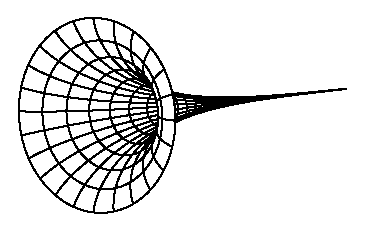
\includegraphics{asy/pseudosphere}
\vskip-3mm
\end{wrapfigure}

Случай $y=e^{-s}$ в \ref{SHORT.ex:principal-revolution:pseudosphere} показан на рисунке; это так называемая \index{псевдосфера}\emph{псевдосфера}.

\begin{thm}{Упражнение}\label{ex:catenoid-is-minimal}
Покажите, что \index{катеноид}\emph{катеноид}, заданный уравнением
\[(\cosh z)^2=x^2+y^2\]
является минимальной поверхностью.
\end{thm}

}

\begin{thm}{Упражнение}\label{ex:helicoid-is-minimal}
Покажите, что \index{геликоид}\emph{геликоид}, определяемый следующей параметризацией
\[s(u,v)=(u\cdot \sin v,u\cdot \cos v,v)\]
является минимальной поверхностью.
\end{thm}

\begin{wrapfigure}{r}{51 mm}
\vskip-6mm
\centering
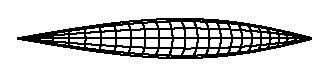
\includegraphics{asy/sin-mini}
\vskip0mm
\end{wrapfigure}

\begin{thm}{Упражнение}\label{ex:rev(sin)}
Пусть $\Sigma$ --- поверхность вращения вокруг оси $x$
с образующей $y=a\cdot \sin x$ для постоянной $a>0$ и $x\in (0,\pi)$.
Покажите, что гауссова кривизна $\Sigma$ не превышает 1.
\end{thm}

\begin{thm}{Упражнение}\label{ex:rev(lin)}
Пусть $f\:(a,b)\to\mathbb{R}$ --- гладкая положительная функция, а $\Sigma$ --- поверхность вращения графика $y=f(x)$ вокруг оси $x$.
Предположим, что $\Sigma$ имеет нулевую гауссову кривизну.
Покажите, что $f$ является линейной функцией; то есть $f(x)=c\cdot x+d$ для некоторых констант $c$ и $d$.
\end{thm}


\section{Аквариум Лагунова}
\index{аквариум Лагунова}

Давайте начнём трёхмерного варианта задачи о луне в луже (\ref{thm:moon}).

\begin{thm}{Вопрос}\label{quest:lagunov}
Предположим, что тело $V\subset \mathbb{R}^3$ ограничено замкнутой поверхностью $\Sigma$ с 
главными кривизнами не больше 1 по абсолютной величине.
Верно ли, что $V$ содержит шар радиуса~1?
\end{thm}

\begin{thm}{Упражнение}\label{ex:moon-revolution}
Покажите, что для тел вращения ответ на вопрос \ref{quest:lagunov} положителен.
\end{thm}

Позже (в \ref{ex:convex-lagunov}) мы увидим, что для выпуклых тел ответ тоже положительный,
а сейчас мы построим пример Владимира Лагунова \cite{lagunov-1961}, показывающий, что в общем случае ответ отрицательный.

\parbf{Построение.}
Начнём с тела вращения $V_1$, поперечное сечение которого показано на следующем рисунке.
Граница поперечного сечения состоит из 6 длинных горизонтальных отрезков, включённых в 3 простые замкнутые гладкие кривые.
(При их построении надо использовать процедуру сглаживания из \ref{sec:analysis}.)
Граница $V_1$ состоит из трёх гладких сфер.

\begin{figure}[hb!]
\centering
\includegraphics{mppics/pic-33}
\vskip0mm
\end{figure}

Мы предполагаем, что кривизна кривых не превышает~1.
Более того, за исключением почти горизонтальных частей, эта кривизна близка к 1.
Самое толстое место в теле $V_1$ там, где все три граничных сферы подходят близко друг к другу;
остальная часть $V_1$ предполагается очень тонкой.
Можно добиться того, чтобы радиус $r$ максимального шара в $V_1$ только чуть превышал $r_2=\tfrac2{\sqrt{3}}-1$.
(Маленький чёрный круг на рисунке имеет радиус $r_2$, если три больших круга единичные.)
В частности, можно считать, что $r<\tfrac16$.

Упражнение \ref{ex:principal-revolution} приводит формулы для главных кривизн применимых к граничным сферам $V_1$;
из них следует, что обе главные кривизны не превышают 1 по абсолютной величине.

\begin{wrapfigure}{o}{21 mm}
\vskip-0mm
\centering
\includegraphics{mppics/pic-910}
\vskip0mm
\end{wrapfigure}

Остаётся сделать границу $V_1$ связной, не испортив при этом оценки главные кривизны и не изменив максимальный радиус шаров внутри тела.

Каждая граничная сфера содержит два плоских круга; они образуют три пары, лежащие близко друг к другу.
Просверлим дыру через две такие пары и соединим отверстия трубкой --- телом вращения, ось которого смещена, но остаётся параллельной оси $V_1$.
Пусть $V_2$ --- полученное тело; его поперечное сечение показано на рисунке.

Теперь повторим операцию для двух других пар кругов.
Пусть $V_3$ --- полученное тело.

Заметим, что граница $V_3$ связана.
Предполагая, что отверстия большие, можно добиться, чтобы её главные кривизны по-прежнему не превышали 1; последнее доказывается так же, как для~$V_1$.
\qeds

Оценка $r_2=\tfrac2{\sqrt{3}}-1$ оптимальна;
это и прочее было доказано Владимиром Лагуновым и Абрамом Фетом \cite{lagunov-1960, lagunov-fet-1963, lagunov-fet-1965}.

\begin{wrapfigure}{o}{55 mm}
\centering
\vskip-0mm
\includegraphics{mppics/pic-920}
\vskip0mm
\end{wrapfigure}

Поверхность $V_3$ в аквариуме Лагунова имеет род 2; то есть её можно параметризовать сферой с двумя ручками.

Действительно, граница $V_1$ состоит из трёх гладких сфер.

При первом сверлении, мы получаем четыре дырки --- две сферы получают по одной дырке, и одна сфера две дырки.
Соединив две сферы трубкой, получаем одну сферу.
При соединении двух дырок оставшейся сферы, получаем тор.
Он изображён слева на рисунке.
Таким образом, $V_2$ ограничено сферой и тором.

Чтобы построить $V_3$ из $V_2$, мы делаем тор из оставшейся сферы и соединяем его трубкой с другим тором, и получается сфера с двумя ручками.

\begin{thm}{Упражнение}\label{ex:lagunov-genus4}
Измените построение Лагунова так, чтобы граничная поверхность была сферой с четырьмя ручками.
\end{thm}


%Recall that Lagunov's fishbowl contains a ball of radius $r_2=\tfrac2{\sqrt{3}}-1$.
%It turns out that this radius is optimal.
%Moreover, \textit{suppose a connected body $V\subset \mathbb{R}^3$ is bounded by a finite number of closed smooth surfaces with principal curvatures bounded by~1.
%Assume $V$ does not contain a ball of radius $r_2$.
%Then the boundary of $V$ has two diffeomorphic connected components.}
%Such $V$ could be the region squeezed between two close surfaces; for example, a region between two concentric spheres.

%For bodies bounded by a sphere, there is a better bound $r_3=\sqrt{\tfrac32}-1$;
%it is the radius of the smallest sphere tangent to four unit spheres that are tangent to each other.
%Note that $r_3>r_2$.
%\textit{If a body $V\subset \mathbb{R}^3$ is bounded by a smooth sphere with principal curvatures bounded  by~1.
%Then $V$ contains a ball of radius~$r_3$.
%Moreover, this bound is sharp; that is, for every $\epsilon>0$, there are examples of such $V$ not containing a ball of radius $r_3+\epsilon$.}

